\documentclass[xcolor=pdftex,dvipsnames,table]{beamer}
 \usetheme{Warsaw}
 \usecolortheme[RGB={0,44,118}]{structure}
% \usefonttheme{structurebold}
 %\useoutertheme{smoothbars}
 \useinnertheme{rounded}
\usepackage{amsfonts}
\usepackage{amsmath}
\usepackage{amssymb}
\usepackage{amsthm}
\usepackage{setspace}
\usepackage{graphicx}
\usepackage{url}
\usepackage{mathtools}
\usepackage[]{algorithmicx}
\usepackage{algorithm}
\usepackage{algpseudocode}
\usetheme{Warsaw}
%\usecolortheme{beaver}

\setbeamertemplate{theorems}[numbered]

\theoremstyle{plain}
\newtheorem{thm}{Theorem}[section]
\newtheorem{cor}[thm]{Corollary}
\newtheorem{lem}[thm]{Lemma}
\newtheorem{prop}[thm]{Proposition}

\theoremstyle{definition}
\newtheorem{defn}{Definition}[section]
\newtheorem{defns}{``Definition"}[section]

\newcommand{\ap}{\ensuremath{\swarrow\,\searrow}}
\newcommand{\nr}{\ensuremath{\swarrow\,\,\,\,\,\,\,\,\,}}
\newcommand{\pl}[1]{\ensuremath{\textup{Li}_#1}}
\setlength{\tabcolsep}{0pt}

\def\CC{\mathbb{C}}
\def\RR{\mathbb{R}}
\def\ZZ{\mathbb{Z}}
\def\NN{\mathbb{N}}
\def\QQ{\mathbb{Q}}
\def\FF{\mathbb{F}}
\def\KK{\mathbb{K}}

\newcommand{\set}[1]{\lbrace #1 \rbrace}
\newcommand{\paren}[1]{\left( #1 \right)}
\newcommand{\brac}[1]{\left[ #1 \right]}
\newcommand{\angl}[1]{\langle #1 \rangle}
\newcommand{\abs}[1]{\left| #1 \right|}

\begin{document}

\title[Elliptic Curves] % (optional, only for long titles)
{Elliptic Curves}
%\subtitle{Text Here}
\author[McCarthy] % (optional, for multiple authors)
{Matthew McCarthy}
\institute[CNU] % (optional)
{
  Christopher Newport University
}
\date[11/14/15] % (optional)
{CNU Math Contest\\ November 2015}

%\subject{Mathematics}

\frame{\titlepage}

\frame{\tableofcontents}

\section[Definitions]{Definitions}

\subsection[Algebraic Structures]{Algebraic Structures}

\begin{frame}
	\frametitle{Groups}
	
	\begin{defn}[Group]
		Let $G$ be a nonempty set and $*:G^2\rightarrow G$ be a binary operation.
		Then $(G,*)$ form a \textit{group} if and only if all of the following are satisfied:
		\begin{enumerate}
			\item there exists an $e\in G$, called the identity, such that for all $g\in G$, $g*e=e*g=g$;
			\item for all $f,g,h\in G$, $f*(g*h)=(f*g)*h$;
			\item for each $g\in G$, there exists an $h\in G$ such that $g*h=h*g=e$, we call $h$ the inverse of $g$, denoted $h=g^{-1}$.
		\end{enumerate}
	\end{defn}
\end{frame}

\begin{frame}
	\frametitle{Abelian Groups}
	\begin{defn}[Abelian Group]
		Let $(G,*)$ be a group. We say that $(G,*)$ is \textit{abelian} if and only if for all $g,h\in G$, $g*h=h*g$.
	\end{defn}
	
	Ex: 
	\begin{itemize}
		\item $(\RR,+)$
		\item $(\CC\setminus\set{0},\cdot)$
		\item $(\ZZ_n,+)$ for $n\in\NN$
		\item $(\ZZ_p\setminus\set{0}, \cdot)$ where $p$ is prime
	\end{itemize}
\end{frame}

\begin{frame}
	\frametitle{Fields}
	
	\begin{defn}[Field]
		Let $\FF$ be a non-empty set and let $+:\FF^2\rightarrow\FF$ and $\cdot:\FF^2\rightarrow\FF$ be binary operations.
		Then $\FF$ is a field if and only if all of the following are satisfied:
		\begin{enumerate}
			\item $(\FF,+)$ forms an Abelian group with identity 0;
			\item $(\FF\setminus\set{0},\cdot)$ forms an Abelian group with identity 1;
			\item for all $x,y,z\in\FF$, $x(y+z)=xy+xz$.
		\end{enumerate}
	\end{defn}
	
	Some examples are $\QQ$, $\RR$, $\CC$, and $\ZZ_p$ where $p$ is prime.
\end{frame}

\subsection[Elliptic Curves]{Elliptic Curves}

\begin{frame}
	\frametitle{Working Definition of an Elliptic Curve}
	
	\begin{defns}[Elliptic Curve (from \cite{AEC})]
		An \textit{elliptic curve} over a field $\FF$ is a nonsingular cubic equation of the form
		\begin{equation}\label{WEQN}
		y^2+a_1xy+a_3y=x^3+a_2x^2+a_4x+a_6
		\end{equation}
		where $a_1,a_2,a_3,a_4,a_6\in\FF$.
	\end{defns}
	\begin{defn}
		An equation of the form of Equation \autoref{WEQN} is called a \textit{Weierstrass equation}.
	\end{defn}
\end{frame}

\begin{frame}
	\frametitle{Nonsingular Curves}
	
	Let $E$ be a curve over a field $\FF$ given by the Weierstrass equation
	\[
	E:\,y^2+a_1xy+a_3y=x^3+a_2x^2+a_4x+a_6.
	\]
	Define
	\begin{align*}
	b_2 & = a_1^2 + 4a_2\\
	b_4 & = a_1a_3+2a_4 \\
	b_6 & = a_3^2 +2a_6 \\
	b_8 & = b_2a_6-a_1a_3a_4+a_2a_3^2-a_4^2\\
	\Delta & = -b_2^2b_8-8b_4^3-27b_6^2+9b_2b_4b_6.
	\end{align*}
	Then $E$ is nonsingular if and only if $\Delta\neq 0$ \cite{AEC}.
\end{frame}

\begin{frame}
	\frametitle{Kinds of Elliptic Curves over $\RR$}
	\begin{columns}
	\column{0.3\textwidth}
	\begin{figure}
		\centering
		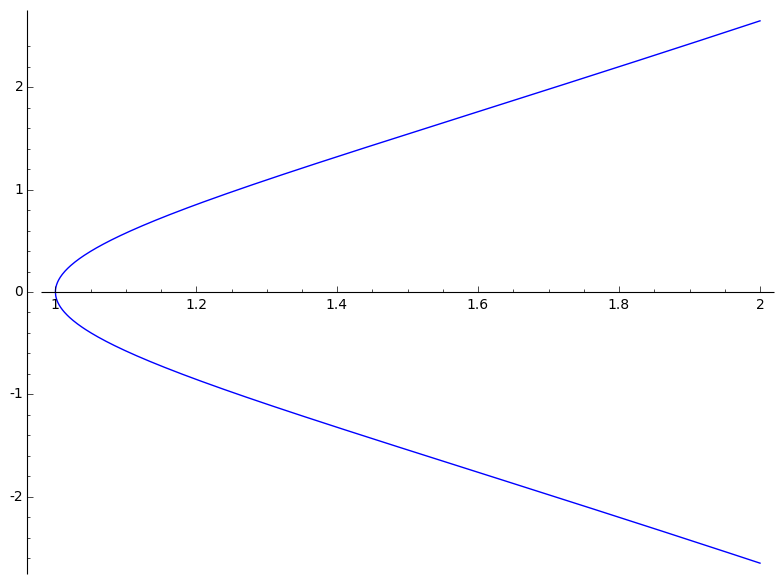
\includegraphics[scale=0.1]{c1.png}
		\caption{$y^2=x^3-1$}
	\end{figure}
	\begin{figure}
		\centering
		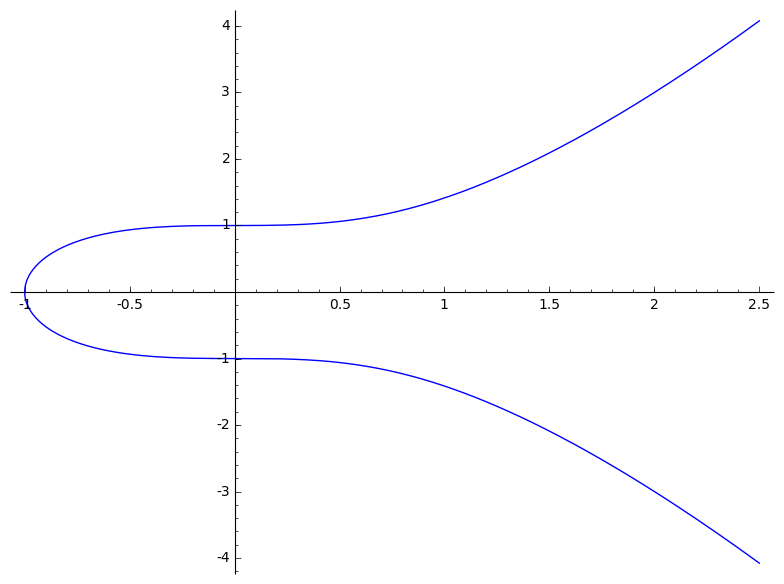
\includegraphics[scale=0.1]{c2.png}
		\caption{$y^2=x^3+1$}
	\end{figure}
	\column{0.3\textwidth}
	\begin{figure}
		\centering
		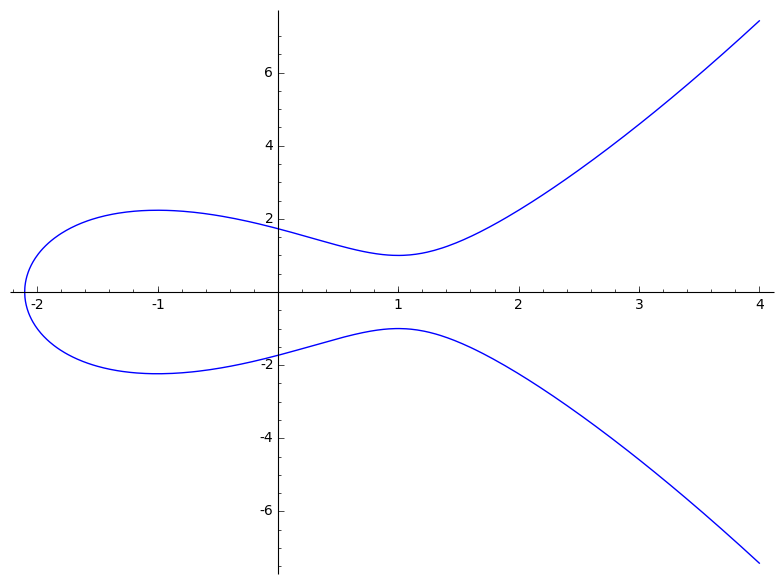
\includegraphics[scale=0.1]{c3.png}
		\caption{$y^2=x^3-3x+3$}
	\end{figure}
	\begin{figure}
		\centering
		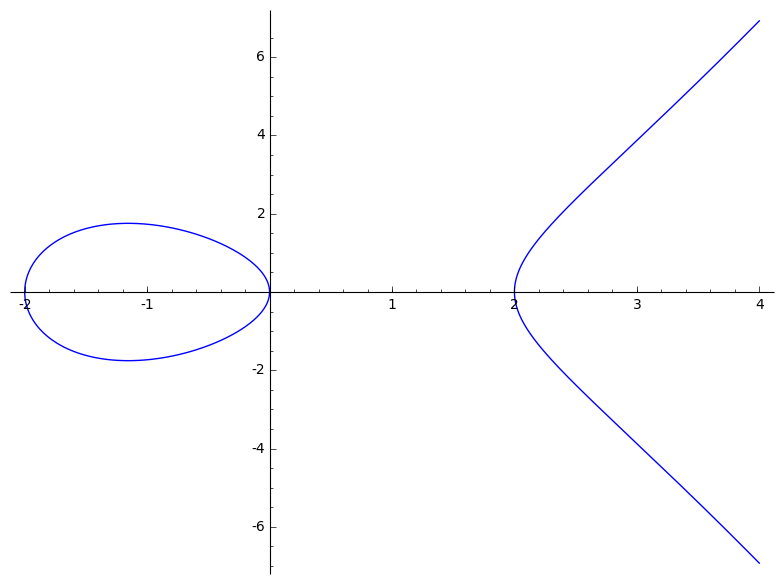
\includegraphics[scale=0.1]{c4.png}
		\caption{$y^2=x^3-4x$}
	\end{figure}
	\column{0.3\textwidth}
	\begin{figure}
		\centering
		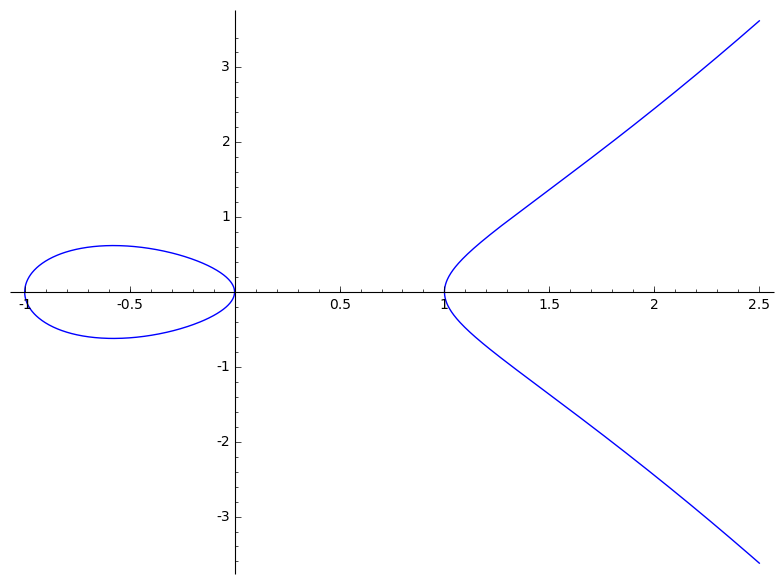
\includegraphics[scale=0.1]{c5.png}
		\caption{$y^2=x^3-x$}
	\end{figure}
	\end{columns}
\end{frame}

\begin{frame}
	\frametitle{Point at Infinity}
	
	Let $E$ be an elliptic curve over a field $\FF$.
	Consider the homogeneous version of $E$'s Weierstrass equation.
	\begin{equation}\label{PWEQN}
	y^2z+a_1xyz+a_3yz^2=x^3+a_2x^2z+a_4xz^2+a_6z^3
	\end{equation}
	Taking $z=x=0$, yields the tautology $0=0$.
	
	Therefore the point $(0:1:0)\in E$.
	
	We say $(0:1:0)$ is the point at infinity.	
\end{frame}

\section[The Group Law]{The Group Law}

\begin{frame}
	\frametitle{Chord and Tangent Rule}
	
	An elliptic curve over a field forms a group under the chord and tangent rule \cite{Galbraith}.
	\begin{columns}
	\column{0.3\textwidth}
	\begin{figure}
		\centering
		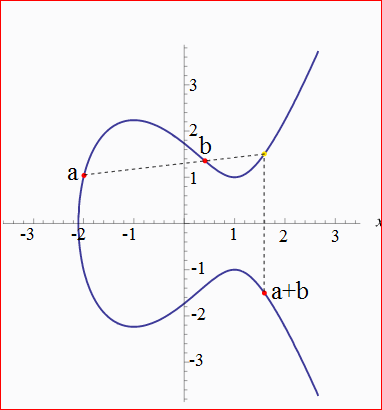
\includegraphics[scale=.3]{p_plus_q.png}
		\caption{$P+Q$}
	\end{figure}
	
	\column{0.3\textwidth}
	\begin{figure}
		\centering
		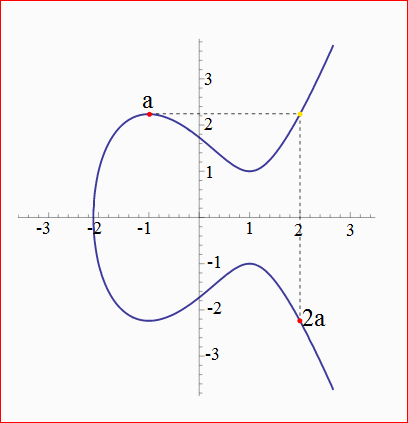
\includegraphics[scale=.3]{p_plus_p.png}
		\caption{$2P$}
	\end{figure}
	\end{columns}
\end{frame}

\begin{frame}
	\frametitle{The Group Law}
	
	\begin{thm}[Group Law (from \cite{AEC})] \label{GL1}
		Let $E$ be an elliptic curve over a field $\FF$ satisfying a Weierstrass equation
		\[
		y^2+a_1xy+a_3y=x^3+a_2x^2+a_4x+a_6.
		\]
		Let $P=(x,y)\in E$.
		Then $-P=(x,-y-a_1x-a_3)\in E$.
		Let $P_1=(x_1, y_1), P_2=(x_2,y_2)\in E$.
		Then $P_1+P_2=P_3\in E$.
	\end{thm}
\end{frame}

\begin{frame}
	\frametitle{The Group Law (Continued)}
	If $x_1=x_2$ and $y_1+y_2+a_1x_2+a_3=0$ then $P_3=\mathcal{O}$.
	Otherwise let $\lambda$ and $\nu$ be described as in the table below.
	\[
	\begin{array}{c|cc}
	& \lambda & \nu\\\hline\\[.2em]
	x_1\neq x_2 & \displaystyle \frac{y_2-y_1}{x_2-x_1} & \displaystyle\frac{y_1x_2 - y_2x_1}{x_2-x_1}\\[1.2em]
	x_1=x_2 &  \displaystyle \frac{3x_1^2+2a_2x_1+a_4-a_1y_1}{2y_1+a_1x_1+a_3} & \displaystyle \frac{-x_1^3+a_4x_1+2a_6-a_3y_1}{2y_1+a_1x_1+a_3}
	\end{array}
	\]
	Then $x_3=\lambda^2+a_1\lambda-a_2-x_1-x_2$, $y_3=-(\lambda+a_1)x_3-\nu-a_3$ and $P_3=(x_3,y_3)$.
\end{frame}

\begin{frame}
	\frametitle{Special Class of Curves}
	\begin{itemize}
		\item Let $E$ be an elliptic curve over $\FF_{2^n}$ satisfying
		\[
		y^2+xy=x^3+a_2x^2+a_6
		\]
		with $a_6\neq 0$.
		
		\item $\FF_{2^n}$ is characteristic 2: for each $\alpha\in\FF_{2^n}$, $\alpha+\alpha=0$ and $\alpha=-\alpha$.
		
		\item These curves admit their own version of the group law \cite{IECC}.
	\end{itemize}
\end{frame}

\begin{frame}
	\frametitle{Group Law over $\FF_{2^n}$}
	
	\begin{thm}[Group Law over $\FF_{2^n}$ (from \cite{IECC})] \label{GL2}
		Let $E$ be an elliptic curve over a field $\FF$ satisfying a Weierstrass equation
		\begin{equation}\label{WEQN2}
		y^2+xy=x^3+a_2x^2+a_6.
		\end{equation}
		Let $P=(x,y)\in E$.
		Then $-P=(x,y+x)\in E$.
		Let $P_1=(x_1, y_1), P_2=(x_2,y_2)\in E$.
		Then $P_1+P_2=P_3\in E$.
	\end{thm}
\end{frame}

\begin{frame}
	\frametitle{Group Law over $\FF_{2^n}$ (Continued)}
	
	If $x_1=x_2$ and $y_1+y_2+x_2=0$ then $P_3=\mathcal{O}$.
	Otherwise let $\lambda,\, x_3,$ and $y_3$ be described as in the table below.
	\[
	\begin{array}{c|ccc}
	& \lambda & x_3 & y_3\\\hline\\[.1em]
	P_1\neq P_2 & \displaystyle \frac{y_2-y_1}{x_2-x_1} & \lambda^2+\lambda+x_1+x_2+a_2 & \lambda(x_1+x_3)+y_1+x_3 \\[1.2em]
	P_1=P_2 &  \displaystyle \frac{y_1}{x_1}+x_1 & \lambda^2+\lambda+a_2 & x_1^2+(\lambda+1)x_3
	\end{array}
	\]
	Then $P_3=(x_3,y_3)$.
\end{frame}

\subsection[Point Operations]{Point Operations}

\begin{frame}
	\frametitle{Point Operations}
	
	Let $E$ be an elliptic curve over $\FF_{2^n}$ and let $P,Q\in E$.
	\begin{itemize}
		\item If $P\neq Q$, then computing $P+Q$ is said to be adding $Q$ to $P$.
		\begin{itemize}
			\item Cost of $P+Q$: $1R+3M$.
		\end{itemize}
		\item Computing $P+P$ is said to be doubling $P$, denoted $2P$.
		\begin{itemize}
			\item Cost of $2P$: $1R+4M$.
		\end{itemize}
		\item Computing $\sum_{i=1}^m P$ is said to be multiplying $P$ by $m$, denoted $mP$.
		\begin{itemize}
			\item To compute $mP$ we use the double and add algorithm.
		\end{itemize}
	\end{itemize}
\end{frame}

\begin{frame}
	\frametitle{Double and Add Algorithm}
	Let $E$ be an elliptic curve over a field $\FF$. 
	Let $P\in E$ and let $n\in\ZZ$.
	\begin{algorithmic}
		\Function{DoubleAdd}{$n\in\ZZ$, $P\in E$}
		\If{$n=0$}
		\State \Return{$\mathcal{O}$}
		\ElsIf{$n=1$}
		\State \Return{$P$}
		\ElsIf{$n<0$}
		\State \Return{ \Call{DoubleAdd}{$-n$, $-P$}}
		\ElsIf{$n\equiv_2 0$}
		\State \Return{$2$ \Call{DoubleAdd}{$n/2$, $P$}}
		\Else
		\State \Return{ $P$ $+2$ \Call{DoubleAdd}{$(n-1)/2$, $P$}}
		\EndIf
		\EndFunction
	\end{algorithmic}
\end{frame}

\section[The Result]{The Result}

\subsection[Framework]{Framework}

\begin{frame}
	\frametitle{Starting Points}
	
	\begin{itemize}
		\item Let $E$ be an elliptic curve over $\FF_{2^n}$ satisfying 
		\[
		y^2+xy=x^3+a_2x^2+a_6
		\]
		with $a_6\neq 0$.
		
		\item Thus, Theorem \autoref{GL2} applies.
		
		\item Let $P_0=(x_0,y_0)\neq\mathcal{O}$ be a point on $E$.
		
		\item We want to compute $2^k P$ for any $k\in\NN$.
	\end{itemize}
\end{frame}

\begin{frame}
	\frametitle{Framework}
	
	\begin{itemize}
		\item Let $P_1 = 2P_0$ and let $P_{j+1}=2P_j$.
		\item $P_j=2^j P_0$
		\item Supposing $P_j\neq\mathcal{O}$, denote $x_j=x(P_j)$ and $y_j=y(P_j)$.
		\item When $^2k \leq|P|$, computing $2^kP$ requires $k$ point doublings.
		\begin{itemize}
			\item $|P|$ denotes the order of $P$, the minimal $m$ such that $mP=\mathcal{O}$.
		\end{itemize}
	\end{itemize}
	
\end{frame}

\begin{frame}
	\frametitle{Framework (Continued)}
	
	After $j$ steps, the point we will double is $P_j$.
	The group law implies following about $P_{j+1}$ assuming $x_j\neq 0$:
	\begin{align}
	\lambda_{j+1}&=\frac{y_j}{x_j}+x_j\label{eqnlmb}\\
	x_{j+1}&=\lambda_{j+1}^2+\lambda_{j+1}+1\label{eqnx}\\
	y_{j+1}&=x_j^2+(\lambda_{j+1}+1)x_{j+1}\label{eqny}.
	\end{align}
	If $x_j=0$, then $P_{j+1}=\mathcal{O}$.
\end{frame}

\begin{frame}
	\frametitle{Framework (Continued)}
	
	By replacing the $y$ terms in the equation for $\lambda$, we gain a recursion solely in $x$ and $\lambda$.
	\begin{equation}
	\lambda_{j+1}=\frac{y_j}{x_j}+x_j=\frac{x_{j-1}^2+(\lambda_j+1)x_j}{x_j}+x_j=\frac{x_{j-1}^2}{x_j}+x_j+\lambda_j+1\label{eqnlmb2}.
	\end{equation}
	
	%We now only need to compute the final $y$ term, and the only $y$ term necessary to find $2^kP$ is $y_0$.
	We now only need to compute the final $y$ term.
	
	This means we can skip computing the middle $k-1$ $y$ terms.
\end{frame}

\subsection[Statement]{Statement}

\begin{frame}
	\frametitle{Calculation of $2^kP$}
	
	\begin{thm} \label{2kP}
		Let $E$ be an elliptic curve over $\FF_{2^n}$ satisfying \autoref{WEQN2} and let $P\neq\mathcal{O}$ be a point on $E$.
		Denote $x_0=x(P)$ and $y_0=y(P)$.
		Then the following algorithm will compute $Q=2^k P$.
	\end{thm}
\end{frame}

\begin{frame}
	\frametitle{Calculation of $2^kP$}
	\begin{columns}[T]
		\column{0.4\textwidth}
		\begin{algorithmic}
		\If{$k=0$}
		\State $Q\gets P$
		\EndIf
		\State $\displaystyle \lambda_1\gets\frac{y_0}{x_0}+x_0$
		\State $\displaystyle x_1 \gets \lambda_1^2+\lambda_1+a_2$
		\If{$x_1=0$}
		\State $Q\gets\mathcal{O}$
		\EndIf
		\State $j \gets 2$
		\end{algorithmic}
		\column{0.6\textwidth}
		\begin{algorithmic}
		\While{$j\leq k$}
		\If{$x_{j-1}=0$}
		\State  $Q\gets\mathcal{O}$
		\EndIf
		\State $\displaystyle \lambda_j\gets\frac{x_{j-2}^2}{x_{j-1}}+x_{j-1}+\lambda_{j-1}+1$
		\State $x_j\gets \lambda_j^2+\lambda_j+a_2$
		\State $j\gets j+1$
		\EndWhile
		\State $y_k\gets x_{k-1}^2+(\lambda_{k}+1)x_k$
		\State $Q\gets(x_k,y_k)$
		\end{algorithmic}
	\end{columns}
\end{frame}

\subsection[Proof]{Proof}
\begin{frame}
	\frametitle{Proof}
	
	\textit{Proof:} Proceed via complete induction.
	
	Base case: $k=1$.
	
	Suppose $x_0\neq 0$.
	Then 
	\[
	\lambda_1=\frac{y_{0}}{x_{0}}+x_{0}.
	\]

	The formulas for $x_1$ and $y_1$ are as the group law states.

	Suppose $x_0=0$.
	
	We know $x_0=x_0$ and $y_0+y_0+x_0=2y_0=0$.
	
	Ergo, $2P=\mathcal{O}$.
\end{frame}
\begin{frame}
	\frametitle{Proof (Continued)}
	
	Base case: $k=2$.
	
	Suppose $x_1\neq 0$.
	Then 
	\[
	\lambda_{2}=\frac{x_{0}^2}{x_{1}}+x_{1}+\lambda_{1}+1=
	\frac{x_{0}^2+(\lambda_{1}+1)x_{1}}{x_{1}}+x_{1}=\frac{y_{1}}{x_{1}}+x_{1}
	\]
	
	The formulas for $x_2$ and $y_2$ are as the group law states.
	
	Suppose $x_1=0$.
	
	We know $x_1=x_1$ and $y_1+y_1+x_1=2y_1=0$.
	
	Ergo, $2^2P=\mathcal{O}$.
\end{frame}
\begin{frame}
	\frametitle{Proof (Continued)}
	
	Assume the modified double and algorithm computes $2^kP$ correctly for all $j\leq 2^{k}$.
	
	Suppose $x_k\neq 0$.
	Then 
	\[
	\lambda_{k+1}=\frac{x_{k-1}^2}{x_{k}}+x_{k}+\lambda_{k}+1=
	\frac{x_{k-1}^2+(\lambda_{k}+1)x_{k}}{x_{k}}+x_{k}=\frac{y_{k}}{x_{k}}+x_{k}
	\]
	
	The formulas for $x_{k+1}$ and $y_{k+1}$ are as the group law states.
	
	Suppose $x_k=0$.
	
	We know $x_k=x_k$ and $y_k+y_k+x_k=2y_k=0$.
	
	Ergo, $2^{k+1}P=\mathcal{O}$. 
	{\flushright\qed}
\end{frame}

\begin{frame}
	\frametitle{Modified Double and Add}
	
	\begin{algorithmic}
		\Function{DoubleAdd2}{$m\in\NN$, $P\in E$}
		\If{$m=0$} \Return{$\mathcal{O}$}
		\ElsIf{$m=1$} \Return{$P$}
		\EndIf
		\State $j\gets 0$
		\While{$m/2^{j}\equiv 0\mod 2$} $j\gets j+1$
		\EndWhile
		\If{$j>0$}
		\State \Return $2^j$ \Call{DoubleAdd2}{$\displaystyle\frac{m}{2^j}$, $P$}
		\Else
		\State \Return $P+$\Call{DoubleAdd2}{$m-1$, $P$}
		\EndIf
		\EndFunction
	\end{algorithmic}
\end{frame}

\subsection[Cost Analysis]{Cost Analysis}

\begin{frame}
	\frametitle{Framework}
	\begin{itemize}
		\item Let $E$ be an elliptic curve over $\FF_{2^n}$ for some $n\in\NN$ satisfying 
		\[
		y^2+xy=x^3+a_2x^2+a_6.
		\]
		
		\item Let $P\in E$ with $P\neq\mathcal{O}$.
		
		\item Let $m\in\NN$ such that $2\leq m <|P|$.
	\end{itemize}
	
	Goal: find the cost of the modified double and add algorithm.
	
	Approach: count field reciprocals and multiplications.
\end{frame}

\begin{frame}
	\frametitle{Framework (Continued)}
	
	\begin{itemize}
		\item $2\leq m\Rightarrow\exists k\in\NN$ such that $2^k\leq m<2^{k+1}$.
		\item $m$ can be written as
		\[
		m=\sum_{j=0}^k m_j2^j=2^k+m_{k-1}2^{k-1}+\ldots +m_12+m_0.
		\]
		where all $m_j\in\set{0,1}$.
		\item Let $i$ denote the number of ones in $m$'s binary expansion.
		\begin{itemize}
			\item Note: $1\leq i\leq k+1$.
		\end{itemize}
	\end{itemize}
\end{frame}

\begin{frame}
	\frametitle{Cost: Double and Add}
	
	\begin{itemize}
		\item Thus:
		\[
		mP=\sum_{j=0}^k \paren{m_j2^j}P=2^kP+\paren{m_{k-1}2^{k-1}}P+\ldots +\paren{m_12}P+m_0P.
		\]
		
		\item Exactly $i$ terms of $\set{m_j}_{j=0}^k$ are ones.
		
		\item Ergo we will do $i-1$ point additions.
		
		\item Double and add will do exactly $k$ point doublings.
		
		\item Therefore the cost of double and add to compute $mP$ is:
		\[
		c_1(m)=kD+(i-1)A=(k+i-1)R + (4k+3i-3)M.
		\]
	\end{itemize}
\end{frame}

\begin{frame}
	\frametitle{Cost: Computation of $2^kP$}
	\begin{columns}[T]
		\column{0.4\textwidth}
		\begin{algorithmic}
			\If{$k=0$}
			\State $Q\gets P$
			\EndIf
			\State $\displaystyle \lambda_1\gets\frac{y_0}{x_0}+x_0$
			\State $\displaystyle x_1 \gets \lambda_1^2+\lambda_1+a_2$
			\If{$x_1=0$}
			\State $Q\gets\mathcal{O}$
			\EndIf
			\State $j \gets 2$
		\end{algorithmic}
		\column{0.6\textwidth}
		\begin{algorithmic}
			\While{$j\leq k$}
			\If{$x_{j-1}=0$}
			\State  $Q\gets\mathcal{O}$
			\EndIf
			\State $\displaystyle \lambda_j\gets\frac{x_{j-2}^2}{x_{j-1}}+x_{j-1}+\lambda_{j-1}+1$
			\State $x_j\gets \lambda_j^2+\lambda_j+a_2$
			\State $j\gets j+1$
			\EndWhile
			\State $y_k\gets x_{k-1}^2+(\lambda_{k}+1)x_k$
			\State $Q\gets(x_k,y_k)$
		\end{algorithmic}
	\end{columns}
\end{frame}

\begin{frame}
	\frametitle{Cost: Computation of $2^kP$ (Continued)}
	
	\begin{itemize}
		\item One fixed point doubling: 
		\begin{itemize}
			\item $1R+4M$
		\end{itemize}
		\item One iteration through loop:
		\begin{itemize}
			\item $1R+3M$
		\end{itemize}
		\item $k-1$ iterations:
		\begin{itemize}
			\item $(k-1)R+3(k-1)M$
		\end{itemize}
	\end{itemize}
	Total Cost:
	\[
	c_2(2^k)=kR+(3k+1)M
	\]
\end{frame}

\begin{frame}
	\frametitle{Cost: Modified Double and Add}
	
	\begin{prop}
		Let $E$ be an elliptic curve over $\FF_{2^n}$ satisfying \autoref{WEQN2}.
		Furthermore, let $P\neq\mathcal{O}$ be in $E$ and let $m\in\NN$ such that $2\leq m< |P|$, the order of $P$.
		Then the cost of computing $mP$ using the modified double and add is as follows:
		\[
		c_2(m) = \begin{cases}
		(k+i-1)R + (3k+4i -3)M & m\equiv 0 \mod{2}\\
		( k+ i-1)R+(3 k+4i-4)M & m\equiv 1 \mod{2}.
		\end{cases}
		\]
	\end{prop}
\end{frame}

\begin{frame}
	\frametitle{Proof}
	
	\textit{Proof:} Suppose $m$ is even.
	\begin{itemize}
	\item Recall that:
	\[
	m=\sum_{j=0}^k m_j2^j=2^k+m_{k-1}2^{k-1}+\ldots +m_12+m_0.
	\]
	Then $m_0=0$ and $i=|\set{j|m_j=1}|$ is bounded by $1\leq i\leq k$.
	
	\item Let $\set{m_{j_\alpha}}_{\alpha=1}^i$ be the subsequence of $\set{m_j}_{j=0}^k$ containing all $m_j$ where $m_j=1$.
	
	\item Define $j_0=0$.
	
	\item Force the $j_\alpha$ to be in ascending order: $j_\alpha < j_{\alpha+1}$.
	
	\item Therefore $j_i=k$.
	\end{itemize}
\end{frame}

\begin{frame}
	\frametitle{Proof (Continued)}
	
	\begin{itemize}
		\item We see that
		\[
		m=\sum_{\alpha=1}^{i}2^{j_\alpha}
		\]
		
		\item Define:
		\begin{equation}\label{recursion}
			S_\beta = \sum_{\alpha=\beta+1}^{i} 2^{j_\alpha -j_\beta}.
		\end{equation}
		Immediately, we have
		\begin{equation}\label{revRecursion}
			S_\beta = 2^{j_{\beta+1}-j_\beta} (S_{\beta+1}+1).
		\end{equation}
		and	$S_0=m$. 
	\end{itemize}
\end{frame}

\begin{frame}
	\frametitle{Proof (Continued)}
	
	From
	\[
	S_\beta = 2^{j_{\beta+1}-j_\beta} S_{\beta+1} +1.
	\]
	we get,
	\[
	S_\beta P = S_{\beta+1}\paren{2^{j_{\beta+1}-j_\beta}P  +P}.
	\]
	
	By counting we see
	\[
	c_2(S_\beta)=c_2(S_{\beta+1})+ \brac{(j_{\beta+1}-j_\beta)R + (3(j_{\beta+1}-j_\beta)+1)M}+\brac{1R+3M}.
	\]
	Claim:
	\[
	c_2(S_{i-\beta})=( (k-j_{i-\beta})+ (\beta -1) )R+(3( k-j_{i-\beta} )+4(\beta-1)+1 )M. 
	\]
\end{frame}

\begin{frame}
	\frametitle{Proof (Continued)}
	
	Proceed via induction.
	
	Base case: $\beta = 1$.
	
	We know that
	\[
	S_\beta = \sum_{\alpha=\beta+1}^{i} 2^{j_\alpha -j_\beta}.
	\]
	Ergo,
	\[
	S_{i-1}P=\paren{\sum_{\alpha=i}^i2^{j_{\alpha}-j_{i-1}}}P=2^{j_{i}-j_{i-1}}P=2^{k-j_{i-1}}P.
	\]
	Thus,
	\[
	c_2(S_{i-1})=( (k-j_{i-1})+ (1 -1) )R+(3( k-j_{i-1} )+4(1-1)+1 )M. 
	\]
\end{frame}

\begin{frame}
	\frametitle{Proof (Continued)}
	
	Assume:
	\[
	c_2(S_{i-\beta})=( (k-j_{i-\beta})+ (\beta -1) )R+(3( k-j_{i-\beta} )+4(\beta-1)+1 )M. 
	\]
	
	We know 
	\[
	c_2(S_{i-(\beta+1)})=c_2(S_{i-\beta})+ (j_{i-\beta}-j_{i-{\beta+1}}+1)R + (3(j_{i-\beta}-j_{i-(\beta+1)})+4)M.
	\]
	Therefore
	\[
	c_2(S_{i-(\beta+1)})=( (k-j_{i-{\beta+1}})+ \beta)R+(3( k-j_{i-(\beta+1)})+4\beta+1)M.
	\]
\end{frame}

\begin{frame}
	By the inductive hypothesis, we know
	\[
	c_2(S_{i-\beta})=( (k-j_{i-\beta})+ (\beta -1) )R+(3( k-j_{i-\beta} )+4(\beta-1)+1 )M. 
	\]
	Thus,
	\begin{align*}
	c_2(m)=c_2(S_{0})&=( (k-j_{0})+ (i -1) )R+(3( k-j_{0} )+4(i-1)+1 )M\\
	&=( k+ i -1 )R+(3 k+4i-3 )M.
	\end{align*}
	
	Ergo, the proposition works for even $m$.
\end{frame}

\begin{frame}
	Suppose $m$ is odd.
	
	Then $mP=(m-1)P+P$.
	
	Moreover, $m-1$ is even.
	
	Thus,
	\begin{align*}
	c_2(m)&=c_2(m-1)+1A\\
	&=( k+ i-1)R+(3 k+4i-4)M.
	\end{align*}
	
	Therefore, the proposition works for odd $m$. {\flushright\qed}
\end{frame}

\begin{frame}
	\frametitle{Savings}
	
	\begin{cor} \label{savings}
		\begin{equation}
		c_1(m)-c_2(m)=\begin{cases}
		0R + (k-i)M & m\equiv 0\mod{2}\\
		0R + (k-i+1)M & m\equiv 1\mod{2}
		\end{cases}
		\end{equation}
	\end{cor}
	
	\begin{Large}
		\begin{center}
			This is always non-negative!
		\end{center}
	\end{Large}
\end{frame}

\section[Conclusion]{Conclusion}

\begin{frame}
	\frametitle{Why do we care?}
	
	Elements in $\FF_{2^n}$ are equivalence classes of polynomials with coefficients in $\ZZ_2$ modulo the principal ideal generated by any irreducible polynomial of degree $n$, $p(a)$, with coefficients in $\ZZ_2$.
	\[
	\FF_{2^n}=\ZZ_2[a]/(p(a))
	\]
	Multiplication in $\FF_{2^n}$:
	\[
	\paren{\sum_{j=0}^m \alpha_j a^j}\paren{\sum_{i=0}^l \beta_i a^i}\equiv \sum_{k=0}^{m+l} \paren{\sum_{j+i=k} \alpha_j\beta_i}a^k \mod{(p(x))}
	\]
	We need to do polynomial multiplication and polynomial long division.
\end{frame}

\begin{frame}
	\frametitle{Conclusion}
	\begin{itemize}
		\item Applications
		\begin{itemize}
			\item Immediately provides fewer field multiplications in any setting.
			\item Cryptography
			\begin{itemize}
				\item Public keys with more zeros $\Rightarrow$ faster enc./dec.
			\end{itemize}
		\end{itemize}
		\item Further research
		\begin{itemize}
			\item Solve the recursion for $\lambda$:
			\[
			\lambda_{j+1}=\frac{\paren{\lambda_{j-1}^2+\lambda_{j-1}+1}^2}{\lambda_{j}^2+\lambda_{j}+1}+\lambda_{j}^2.
			\]
			
			\item Investigate methods for quickly computing $\alpha^kP$.
			
			\item Investigate methods for quickly computing $2^{-k}P$ (see \cite{ECDSA}).
		\end{itemize}
	\end{itemize}
	
\end{frame}

\begin{frame}[allowframebreaks]
\frametitle{References}
\begin{thebibliography}{10}    
	\bibitem{Galbraith}
		Steven D. Galbraith
		\newblock Mathematics of Public Key Cryptography
	\bibitem{ECDSA}
		Richard Schroeppel and Cheryl Beaver
		\newblock Algorithms for Improved Performance in Cryptographic Protocols
		\newblock Sandia National Laboratories. In: SAND REPORT (2003-4283)a
	\bibitem{AEC}
		Joseph H. Silverman
		\newblock The Arithmetic of Elliptic Curves
		\newblock Graduate Texts in Mathematics
	\bibitem{IECC}
		Micheal Rosing
		\newblock Implementing Elliptic Curve Cryptography
	\bibitem{ET}
		Avner {Ash} and Robert {Gross}
		\newblock Elliptic Tales
\end{thebibliography}
\end{frame}

\begin{frame}
\begin{Large}
\begin{center}
Thank you!
\end{center}
\end{Large}
\end{frame}

\end{document}
